    % Transcription factors are important because they modify the transcriptional machinery
        \subsubsection{Gene Expression}
        Gene expression is crucial to the function and differentiation of various cell types and required for growth, repair and maintenance of an organism.  In eukaryotic cells, DNA is coiled around a protein structure called a histone, forming a nucleosome (see Fig~\ref{fig:chromatin1}); these are collected in tightly packed configurations, known as chromatin, in the nucleus of cells~\cite{alberts2002chromosomal, kornberg1974chromatin}. A gene is a region in the DNA that contains the necessary information for the synthesis of an associated protein. The types of genes that get expressed and the associated intensity in a cell is known as an expression profile. All the nucleated cells in an organism contain the same DNA, but differences in the expression profiles is what gives rise to the different cell types and functions~\cite{lockhart2000genomics}.% In this thesis, our interest lies in the identification and classification of certain regions in the DNA that help regulate the expression of particular family of cardiac genes. %\textbf{That need to be described below}. 

        
            \begin{figure}[H]
                 \centering
            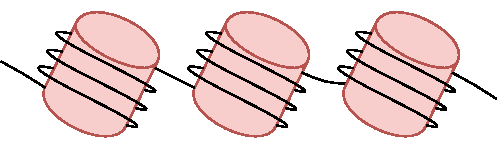
\includegraphics[width=0.5\textwidth]{Chromatin.pdf}
                \caption{The black lines represent DNA and are wrapped around histones, represented by red cylinders. This configuration makes up a nucleosome, which is the basic unit of chromatin.}
                \label{fig:chromatin1}
            \end{figure}
            

        
        
        One of the enduring tenets of molecular biology is that gene expression occurs as a result of DNA being transcribed to RNA and then translated to proteins. Shortly after the discovery of DNA as the carrier for genetic information and the structure of DNA, this process was dubbed the \emph{Central Dogma of Molecular Biology} (see Fig~\ref{fig:centralDogma})~\cite{crick1958protein, macleod1944studies, watson1953structure}. During the first stage of transcription, proteins called transcription factors (TFs) bind to regulatory regions surrounding the gene to recruit RNA polymerase, an enzyme responsible for the synthesis of a sub-type of RNA known as messenger RNA (mRNA). This mRNA is the product of transcription with the purpose of carrying genetic information from the DNA for further processing. In the next phase, molecules called ribosomes, in conjunction with translational RNAs are resposible for the translation of the mRNAs into protein; this second phase is referred to as translation. The proteins are then used for various purposes in the cell, such as maintaining function. %The second phase, known as translation, is primarily carried out by molecules called ribosomes and by translational RNA (tRNA) outside of the nucleus. The ribosomes in conjunction with tRNAsThe end result is a protein comprised of an amino acid chain to be used for cell function.
        
        \begin{figure}
            \centering
            \centering
                \begin{tikzpicture}[node distance=2cm]
                    \node (DNA) [startstop]{DNA};
                    \node (mRNA) [startstop, below of = DNA]{mRNA};
                    \node (Protein) [startstop, below of = mRNA]{Protein};
                    
                    \draw[arrow] (DNA) -- (mRNA);
                    \draw[arrow] (mRNA) -- (Protein);
                    
                    \draw [arrow] (DNA) -- node[anchor=west] {transcribes} (mRNA);
                    \draw [arrow] (mRNA) -- node[anchor=west] {translates} (Protein);
                \end{tikzpicture}
            \caption{The central dogma of molecular biology: DNA is transcribed to make mRNAs, which as subsequently translated in to proteins. (This diagram may be subject to change)}
            \label{fig:centralDogma}
        \end{figure}
        
        % Changes in gene expression can give rise to different outcomes. 
        There are typically two ways that gene expression can be altered.
        %, giving rise to different outcomes; 
             % A type of mutation known as a single nucleotide polymorphism, that is, the substitution of a single nucleotide base for another.
        % The first type of alteration is the direct alteration of the DNA sequence. A mutation in the DNA sequence of a gene can result in the expression of a different genotype.   
        The first type of alteration is the direct modification of the DNA sequence through mutation; this can result in the expression of different genotypes.
        For example, sickle cell anaemia is the result of the mutation of a single nucleotide and affects the haemoglobin carrying capacity of blood cells, causing the sufferer to develop an array of health complications such as strokes~\cite{clancy2008dna}. 
        % This disease is an extreme case of what can go wrong when mutations occur in DNA. 
        Mutations in organisms that lead to expression of genotypes that are beneficial for an organism can be positively selected for in an organism in an appropriate context. Whether a mutation that results in a different genotype is beneficial or not for an organism is context dependent, but this is essentially one of the drivers of evolution. Fortunately, there is typically some redundancy when it comes to the genotype of an organism and mutations considered beneficial in context are often selected for.
        
        The other mechanism for changes in gene expression that will be focused on in this thesis are epigenetic factors. Epigenetics is the study of heritable mechanisms for regulating gene expression that are not linked with direct changes to DNA sequences~\cite{holliday2006epigenetics}. There are many epigenetic factors involved in the process of regulation, such as RNA, acetylation, phosphorylation and more~\cite{geiman2002chromatin, jaenisch2003epigenetic, holoch2015rna, waterland2003transposable}. Each play important roles in the grand scheme of regulating gene expression. 
        
        With the increasing amount of available data that describes gene expression, the modern practice of computational identification for enhancer regions involves the incorporation of various data types. Some example of data types that have been used are conservation \cite{visel2007enhancer}, chromatin profile of histone markers \cite{won2010genome} and chromatin accessibility combined with information about general transcription factor binding sites (TFBS) \cite{boyle2010high}. We are interested in the extension of computational and statistical methods or the development of new ones. Each of these data types provides different information about the state of DNA and the more relevant ones more relevant to this project will be discussed. 
        
        % For the purpose of this report, the way chromatin remodelling, methylation and certain TFs interact discussed in detail since these the interplay between these three factors is what we aim to use in the development of computational models.
        
        \subsubsection{Regulation of Gene Expression}
        
        Protein synthesis is a multi-stage process and regulation can occur at any of the stages. Here a focus will be placed at the transcriptional level.
        Regulation at the transcriptional level requires the orchestrated efforts of a diverse range of factors, proteins and enzymes with a variety of roles. Among these, a notable example are TFs, as the initiation of the transcription and the recruitment of other factors depends on binding interactions between TFs and DNA~\cite{lemon2000orchestrated}. Modifications in the interactions of these factors can affect the expression profile of a cell. The remainder of this report will be devoted to a particular type of TFBS and how come mechanisms for transcriptional regulation affect TF-DNA binding. 
        
        % The modification of the way these factors interact can affect the final expression profile. 
        
        TFBSs are often described as \emph{cis}-regulatory elements (CREs), since they are often found ``in \emph{cis}", that is on the same chromosome that their target gene can be found. These TFBSs are then classified according to their function; either as silencers, promoters, insulators and enhancers~\cite{gaszner2006insulators, gross1988nuclease, li1999locus}. 
        Enhancers are segments of DNA, usually a few 100 base pairs in length, that act as platforms for the recruitment of TFs for the regulation of transcription~\cite{spitz2012transcription}. 
        Regardless of the type of CRE, the main mechanism by which CREs carry out their function is through TFs binding to sequences in the DNA not associated with gene coding, so called non-coding sequences. 
        TFs act by binding in clusters to DNA, but are also thought to form protein complexes known as enhanceosomes, through TF-TF interactions. Spitz and Furlong~\cite{spitz2012transcription} provide a review of some current models for TF-DNA and TF-TF interactions required for the regulation of gene expression.
        
        % Spitz and Furlong~\cite{spitz2012transcription} provide a review of the importance of enhancers and how their interactions with each other to form enhancer complexes and different models of TF-DNA and TF-TF interactions. 
        
        In order for these TFs to bind to DNA, they require access to their target binding sites. As mentioned earlier, DNA is packaged into nucleosomes and subsequently chromatin. Depending on the configuration of the packaging, this may hinder or facilitate the expression of a gene by either limiting or increasing the accessibility to regions of DNA~\cite{li2007role}. Figure~\ref{fig:openclose}(a) shows a schematic of open chromatin that is accessible to TF binding and versus closed chromatin, not accessible tor TF binding in Figure~\ref{fig:openclose}(b). Specific chromatin structures are required to maintain proper gene expression and it has been shown that failure to maintain such proper structure can result in changes in gene expression~\cite{ehrlich2001dna}. Chromatin remodelling is the process of repackaging the chromatin and changing the accessibility to different regions in the DNA. By changing the accessibility of chromatin at different times, cells are able to change their gene expression as is typically seen during tissue development. There are various mechanisms for the remodelling of chromatin, the modification of histone proteins will be discussed.%For example, genes located in closed chromatin can be silenced due to the binding sites required for the intiation of transcription not being able to be reached.

        Histone methylation is the addition of a chemical structural sub-unit known as a methyl group to the tails histone proteins that make up the core of the nucleosomes (red cylinders in Fig~\ref{fig:chromatin1}). This is of interest in this report because the modification of histones is able to influence the chromatin landscape, affecting the DNA interactions with proteins and the stability of gene expression ~\cite{jaenisch2003epigenetic, whetstine2009histone}.
        In fact, enhancer activity has been associated with chromatin signatures comprising different types of histone modifications~\cite{heintzman2007distinct, creyghton2010histone, rada2011unique}.
        DNA found in histone methylated regions are wound tightly around histones are typically transcriptionally silent.
        The remodelling of chromatin through histone methylation can alter the accessibility of transcriptional machinery, allowing TFs to reach their target genes~\cite{gibney2010epigenetics, holoch2015rna}. 

        \begin{figure}[H]
            \centering
            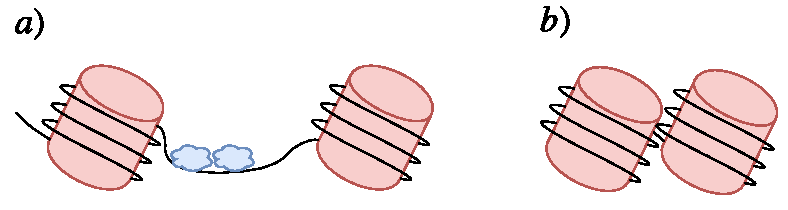
\includegraphics[width=0.9\textwidth]{OpenCloseChromatin.pdf}
            \caption{a) A diagram of open chromatin. TFs, represented by blue cloud shapes are able to access DNA and bind. b) A diagram of closed chromatin. The nucleosomes are tightly packed and the DNA is not accessible to TFs for binding.}
            \label{fig:openclose}
        \end{figure}
        % TBA: spcecificity of heart enhancers and examples

        % We are kinda interested in cardiac tissue because our collaborats are researching this. (Really shallow)
        % FAR OUT. 
        

        % The framework that I propose will be one where we use methylation data, collected by one of of our collaborators, to infer the state of chromatin and subsequently, the motifs of sequences that area candidates for TFBSs that we then compare in an alignment free algorithm.

        
        
        % During transcription, TFs are able to recognize short sequences in non-coding regions of DNA and bind to these sites.
        % Upon binding, TFs recruit other TFs to bind to other sites on the DNA or to the proteins themselves.
        % The exact mechanism of how these TF complexes work is not understood very well. 
        % One plausible explanation is that some combination of TFs need to be succesfuly bound to DNA to carry out their function.
        % Another theory suggests that TFs can bind in a non-specific way to DNA sequences as well as other TFs, introducing 
        % a dimension of protein-protein interaction in to the activation of the reglatory element. 
        % There are other suggestions on how TFs might bind cooperatively in order to become active regulatory elements; for a review, 
        % see Spitz and Furlong (2012)~\cite{spitz2012transcription} for a more in depth explanation. 
        
        % For example, the inhibition of a certain protein required for the initiation of a gene can cause a gene to fail to be expressed. Biogists have used this idea as the basis for protocols used in labs to help design experiments \textbf{THERE SHOULD BE A REFERENCE HERE}. The remainder of this section will be devoted to a more focused explanation of epigenetic factors for gene regulation, relating specific elements to the data provided by collaborators and giving context to the project. 
        % Thus, gene expression is regulated in many stages by a variety of factors. Here, the focus is placed on regulation in the context of transcription.
        
% The main mechanism by which TFs interact with DNA, and subsequently regulate transcription
% . the In this work, we focus on transcriptional regulation, through enhancers.

        


% Here are the main ways that gene expression might be altered:
% \begin{itemize}
% 	\item Direct changes to DNA sequence. 
	
% 	\item Epigenetic changes. Gene expression is a complex and multifaceted process. Regulation in the expression
% 		of a gene happens at different levels, at different stages, by different factors. For the purposes
% 		of this work, a focus will be placed on regulation at the transcriptional level. Specifically, the focuse
% 		will be placed on a subset of TFs. We would like to identify and classify these enhancers at a stage
% 		at a sequence level.
% \end{itemize}

        
        % TF binding sites (TFBS) are divided into categories according to the function associated with the TFs that bind to that site.
        % We would like to focus on the category known as Enhancers. Enhancers are a type of TFBS that enhance or upregulate the 
        % expression of a gene associated with that site.
        % To compount things a single enhancer may act on multiple genes at some distance away from the gene of interest. 


        % ?Changes in gene expression can often be attributed to changes in either the direct genetic sequence (\emph{eg.} mutation), or epigenetic factors in the expression process. There are numerous ways that epigenetic factors can alter the expression of genes without changes to the genetic code itself. A readily available example of an epigenetic factor are TFs. These TFs take on a diverse set of roles in regulating transcription, ~\cite{lemon2000orchestrated}.
        
        % \subsection{Enhancer Identification}
        


         % This denotes the methylation status of a histone. This the methylation of this particular site often associated with promoter regions of actively being transcribed genes~\cite{barski2007high}. 
        %https://epigenie.com/key-epigenetic-players/histone-proteins-and-modifications/histone-h3k4/
        
        
        % The many faces of histone lysine methylation 2002)
        
        % Revisit Spitz and Furlong to see what sort of idease we have to give an overlay of what a TF is and how we have different models for regulation. 

        
        % Changes in gene expression is primarily driven by direct changes in the sequence (genetic) or changes in epigenetic factors involved in the expression process, such as chrmomatin remodelling through histone methylation altering accessibility between transcriptional machinery and their target gene~\cite{gibney2010epigenetics, holoch2015rna }.% (RNA CAN ALSO REGULATE GENE EXPRESSION MAYBE) 
        % Epigenetics is important~\cite{}
        
        
        % A direct alignment based approach might not be the best way since these things display modest or no conservation. 
        
        %  Some of the problems associated with the characterization of enhancer regions are as follows:
        % 	\begin{itemize}
        % 		\item Many enhancers are active at a given time in any given tissue. 
        % 		\item There is a many-to-many correspondence between enhancers and genes. That is, a single enhancer may be acting on multiple genes and each gene may have multiple enhancers acting on it. 
        % 		\item Traditional wet-lab assays can can find only one enhancer at a time. 
        % 	\end{itemize}

        
        % \begin{itemize}
        % 	\item Unsupervised: K-means, HMM
        % 	\item Supervised: Artificial Neural Networks, Decision Trees, Random Forest
        % 	\item Bayesian Segmentation and classification? (What is this)
        % 	\item Alignment Free Sequence comparison 
        % \end{itemize}

        % We have many different 
        % \subsection{How are they found in the wet lab?}
            
        % \subsection{How are they found computationally?}
        
        
        %     So, transcription factors are proteins that can bind to DNA. These proteins are responsible for the initiation and regulation of transcription. Something about gene control comes from regulation. 
            
        %     To speak some of the lingo, these \emph{cis}-regulatory elements can hang out together and create these \emph{modules} that act as the high density binding sites for these elements. Enhancers are segments of DNA, typically a few 100 base pairs in length that act as binding sites for transcription factors that stimulate the transcription of genes. 
            
        %     Enhancer regions are part of the subset of DNA that is considered to be non-coding. 
        %     These regions can be sites for transcription factor binding and are thought to play an important role in stimulating gene expressions. 
        %     {\color{red} The role of enhancers might vary at different developmental stages}
        %     There are competing models proposed about how these enhancer regions work in the recruitment and attraction of transcription factors and how they encourage binding; these are the billboard, the enhanceosome and the TF collective. While they vary in the mechanisms in the activation of the enhancer, they all rely on a binding mechanism for activation.
            
        %     Part of the difficulty in attempting to characterize these enhancer regions is that unlike coding DNA regions, there is no clear pattern underlying these. There have been previous attempts to identify and classify these elements grounded in different bioinformatic, statistical and mathematical frameworks.
            
        %     The most familiar of these would be sequence segmentation and alignment based approaches.
            
        %     In a pairwise sequence alignment, the algorithm requires two input sequences. What you do 







% Check methods that you think are going to in the field. Maybe later in the thesis, have a better idea of the things that you are expecting. 

% Email Sarah. sarah.boyd@monash.edu 

% Include the cursory analysis that we used in changepoint. 

% Be useful to Mirana. Be more autonomous in what I have to do. Perhaps work changepoint in to the theory. Revisit Manjula paper. 

% Going to work a little bit more the cohesion. high CG sequence tend to be functional components. 

% Compare chagnepoint output with histone marks. How does modelling to work. Independence of position, how to incorporate. 

  
  
  
  
  
  
  
  
  
  
  
   % {SOME OF THE PROBLEM THAT WE HAVE WHEN TRYING TO FIND ENHANCERS IS THAT:
        %     \begin{itemize}
        %         \item MANY ENHANCERS ARE ACTIVE AT A GIVEN TIME
        %         \item MANY TO MANY CORRESPONDENCE BETWEEN GENES BEING REGULATED AND ENHANCERS REGULATING
        %         \item WETLAB ASSAYS CAN ONLY FIND LIKE ONE ENHANCER AT A TIME
                
        %     \end{itemize}
        % }

       
        % By turning to more computational approaches to the identification of enhancers, the approach is now using computational tools to identify enhancers and then attempting to verify experimentally in the lab.
        
        % Classification into three types of computational methods:
        % \begin{itemize}
        %     \item Epigenetic signature
        %     \item Mainls Chip Seq- Machine Learning stuff
        %     \item Experimental
        % \end{itemize}
        % Three main approaches to computational identification are
        % 	\begin{itemize}
        % 		\item sequence based 
        % 		\item comparative genomics
        % 		\item using epigenetic marks
        % 	\end{itemize}